\documentclass{article}

% http://bayesiandeeplearning.org/

% if you need to pass options to natbib, use, e.g.:
% \PassOptionsToPackage{numbers, compress}{natbib}
% before loading nips_2018

% ready for submission
\usepackage{nips_2018}

% to compile a preprint version, e.g., for submission to arXiv, add
% add the [preprint] option:
% \usepackage[preprint]{nips_2018}

% to compile a camera-ready version, add the [final] option, e.g.:
% \usepackage[final]{nips_2018}

% to avoid loading the natbib package, add option nonatbib:
% \usepackage[nonatbib]{nips_2018}

\usepackage[utf8]{inputenc} % allow utf-8 input
\usepackage[T1]{fontenc}    % use 8-bit T1 fonts
\usepackage{hyperref}       % hyperlinks
\usepackage{url}            % simple URL typesetting
\usepackage{booktabs}       % professional-quality tables
\usepackage{amsmath}
\usepackage{amsfonts}       % blackboard math symbols
\usepackage{nicefrac}       % compact symbols for 1/2, etc.
\usepackage{microtype}      % microtypography
\usepackage{graphicx}
\usepackage{subcaption}
\usepackage{ownstyles}


% % Commenting highlights
\newif\ifcomments

%Uncomment one of the two lines below to turn todos on/off
%\commentsfalse
\commentstrue

\ifcomments
\newcommand{\comments}[1]{#1}
\else
\newcommand{\comments}[1]{}
\fi
% % Commenting highlights


\title{Metropolitan Generative Adversarial Networks}

% The \author macro works with any number of authors. There are two
% commands used to separate the names and addresses of multiple
% authors: \And and \AND.
%
% Using \And between authors leaves it to LaTeX to determine where to
% break the lines. Using \AND forces a line break at that point. So,
% if LaTeX puts 3 of 4 authors names on the first line, and the last
% on the second line, try using \AND instead of \And before the third
% author name.

\author{
  David S.~Hippocampus\thanks{Use footnote for providing further
    information about author (webpage, alternative
    address)---\emph{not} for acknowledging funding agencies.} \\
  Department of Computer Science\\
  Cranberry-Lemon University\\
  Pittsburgh, PA 15213 \\
  \texttt{hippo@cs.cranberry-lemon.edu} \\
  %% examples of more authors
  %% \And
  %% Coauthor \\
  %% Affiliation \\
  %% Address \\
  %% \texttt{email} \\
  %% \AND
  %% Coauthor \\
  %% Affiliation \\
  %% Address \\
  %% \texttt{email} \\
  %% \And
  %% Coauthor \\
  %% Affiliation \\
  %% Address \\
  %% \texttt{email} \\
  %% \And
  %% Coauthor \\
  %% Affiliation \\
  %% Address \\
  %% \texttt{email} \\
}

\renewcommand{\vec}[1]{{\boldsymbol{\mathbf{#1}}}} % vector
\newcommand{\mat}[1]{{\ensuremath{\mathbf{#1}}}} % matrix

\newcommand{\R}{\mathbb{R}}
\newcommand{\D}{\mathcal{D}}
\newcommand{\N}{\mathcal{N}}
\newcommand{\set}[1]{\mathcal{#1}}

\newcommand{\bigO}{\mathcal{O}}
\newcommand{\ceq}{{\stackrel{c}{=}}}
\newcommand{\half}{\frac{1}{2}}
\newcommand{\T}{^\top}
\newcommand{\I}{\mathbb{I}}

\newcommand{\grad}{\nabla}
\newcommand{\sample}{\sim}
\newcommand{\given}{|}

\newcommand{\norm}{\mathcal{N}}
\newcommand{\bern}{\textrm{Bern}}

\DeclareMathOperator*{\argmin}{argmin}
\DeclareMathOperator*{\argmax}{argmax}

\newcommand{\target}{{p^\star}}
\newcommand{\prop}{q}
\newcommand{\pinit}{{p_0}}

\newcommand{\PG}{{p_G}}
\newcommand{\PD}{{p_D}}
\newcommand{\PR}{{p_R}}
\newcommand{\accept}{\alpha}

\newcommand{\setx}{\set{X}}

% Finish clean up checks:
% TODO use smash where needed
% TODO \! arrow where needed
% TODO can search, it is

% G vs PG

\begin{document}
% \nipsfinalcopy is no longer used

\maketitle

% Do at end
% Might not be needed for workshop since 3 page limit anyway
%\begin{abstract}
%  The abstract paragraph should be indented \nicefrac{1}{2}~inch
%  (3~picas) on both the left- and right-hand margins. Use 10~point
%  type, with a vertical spacing (leading) of 11~points.  The word
%  \textbf{Abstract} must be centered, bold, and in point size 12. Two
%  line spaces precede the abstract. The abstract must be limited to
%  one paragraph.
%\end{abstract}

\section{Introduction}

% GANs provide implicit way to do density estimation
% traditionally done with explicit likelihood, ancestral sampling in most models to get new synthetic data points from fit model
Generative adversarial networks (GANs) presented a radically new way to do density estimation:
They only implicitly represent the density of the data via a classifier that distinguishes real from generated data.
Traditionally, density estimation has been done with a model that can easily compute the likelihood of the observed data.
% TODO or if not, like RBM, could do MCMC method based on likelihood, GAN easy to sample but not likelihood

\todo{test item maybe delete me}
\todo{test item maybe delete me}
\jby{hi}

% GAN uses D and G, but then D usually thrown away
% Use new method to capture knowledge captured in D, to wrap G and create a more intelligent G'
GANs iterate between updating a discriminator $D$ and a generator $G$, where $G$ generates new (synthetic) samples of data, and $D$ attempts to distinguish samples of $G$ from the real data.
Typically, in this setup, $D$ is thrown away at the end of training, and only $G$ is kept for generating new synthetic data points.
In this work we propose the Metropolitan GAN (MGAN) that constructs a new generator $G'$ that ``wraps'' $G$ using the information contained in $D$.
This principle is illustrated in Figure~\ref{fig:block_diag}.

\begin{figure}[bhtp]
    \centering
    \begin{subfigure}[t]{2.25in}
       \centering
       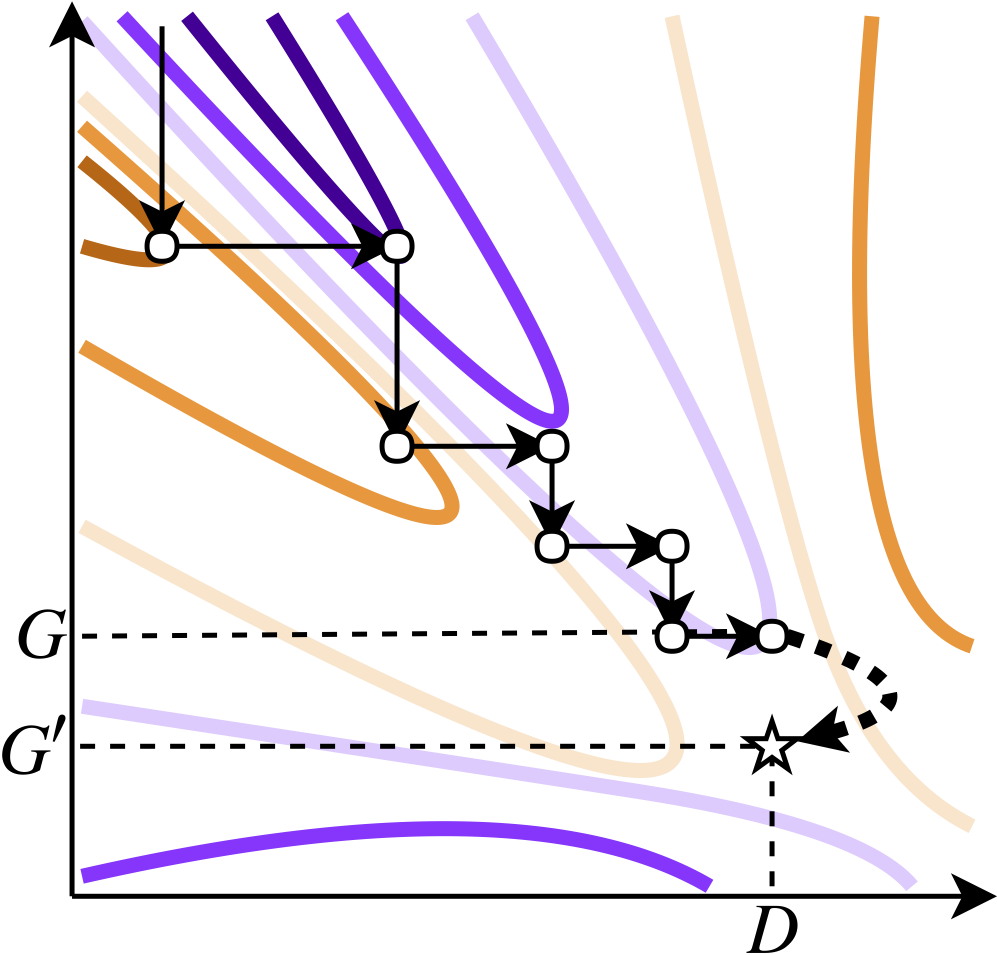
\includegraphics[width=2.25in]{figures/coord_descent.png}
       \caption{GAN objective}
    \end{subfigure}
    \begin{subfigure}[t]{3in}
       \centering
       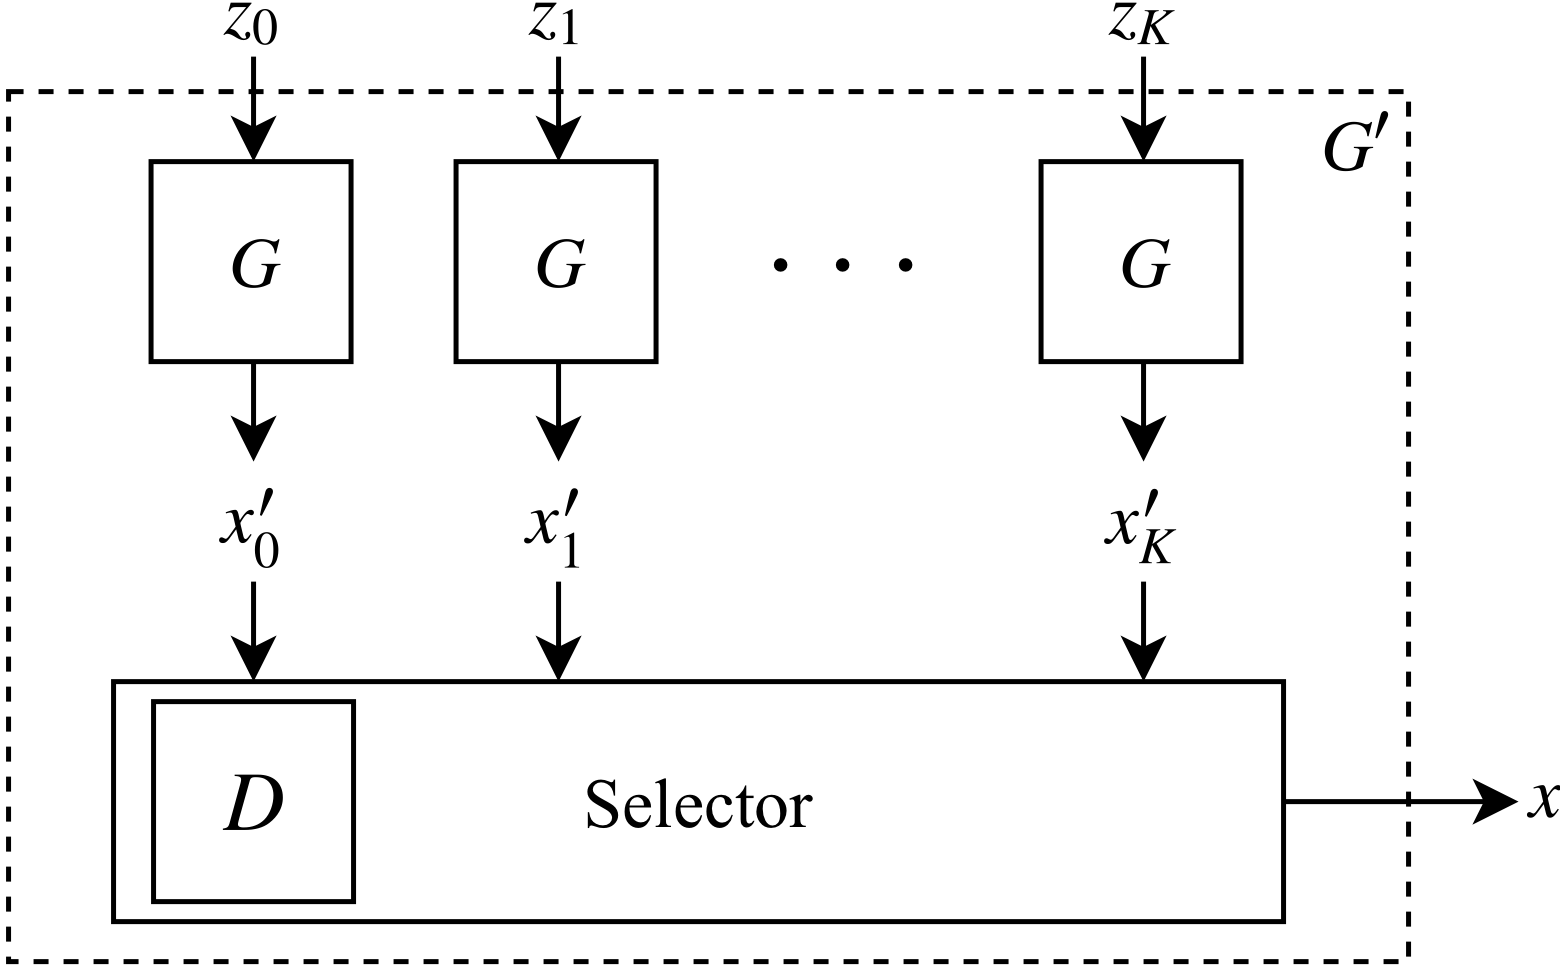
\includegraphics[width=3in]{figures/block_diag.png}
       \caption{$G'$ wraps $G$}
    \end{subfigure}
    \caption{{\small
    On the left we illustate how training of $D$ and $G$ in GANs performs coordinate decsent on the joint minimax objective, shown in the solid black arrow.
    Assuming traditional GAN training can get us close to the optimal $D$, wrapping $G$ with the MGAN gives us the optimal generator $G'$, as shown in the final dashed arrow.
    On the right we illustrate how the MGAN is essentially a selector among multiple draws from $G$.
    In the MGAN, the selector is built using a Metropolis-Hastings acceptance rule (i.e., MCMC) from the discriminator scores $D$.
    }}
    \label{fig:block_diag}
\end{figure}

% Approach is based on notion that we can sample from real distn \PR implied by D that discriminates between \PR
% Corollary is that if D is perfect, but G is good, we can sample from the data generating distn exactly
The MGAN uses Markov chain Monte Carlo (MCMC) methods to sample from the distribution implicitly defined by the discriminator $D$.
This is based on the notion that the discriminator classifies between the generator $G$ and a real data distribution:
\begin{align}
  D(\vec x) = \frac{\PD(\vec x)}{\PD(\vec x) + \PG(\vec x)}\,,
\end{align}
where $\PG$ is the (intractable) density of samples from the generator $G$, and $\PD$ is the real data density implied by the discriminator $D$.
If GAN training reaches its global equilibrium then this discriminator distribution $\PD$ is equal to the true distribution on the data ($\PR = \PD$)~\citep{Goodfellow2014}.

% We use MCMC independence sampler to get samples from \PR using multiple samples from G
% MCMC not directly applicable since the likelihood of \PR and G are not available
% However, MCMC only needs the ratio of \PR/G and this can be found from D
We use an MCMC \emph{independence sampler}~\citep{Tierney1994} to get samples from $\PD$ using multiple samples from $G$ (as the proposal)\@.
As a corollary: Given a perfect discriminator $D$ and a decent (but imperfect) generator $G$, we can obtain exact samples from the true data distribution $\PR$.
Standard MCMC implementations cannot achieve this because MCMC requires (unnormalized) densities for the target $\PD$ and the proposal $\PG$.
Neither of these quantities are available in GANs.
However, MCMC can be performed using only the ratio $\PD / \PG$, which is implied by the discriminator $D$.

% We also avoid the burn in issues usually associated with MCMC
% Typically, we cannot get a good initial sample because sampling over parameter space from posterior
% But in this application we are sampling from data space
% So, if init from true data point, then already at true distn for init, and will stay at true distn as result of detailed balance
% TODO do VAEs make similar kinds of arguments?
We can also avoid the burn-in issues that usually plague MCMC methods.
Recall that via the detailed balance property, if the marginal distribution on a Markov chain state $\vec x \in \setx$ at time step $k$ matches the target $\PD$ ($\vec x_k \sample \PD$) then the marginal at time step $k+1$ will also follow $\PD$ ($\vec x_{k+1} \sample \PD$)\@.
Typically, it is not possible to get an initial sample from the target distribution ($\vec x_0 \sample \PD$) because MCMC is typically applied to generate samples of \emph{parameters} from a Bayesian posterior distribution.
We have no example samples of parameters from these distributions to start from.
However, in MGANs, we are sampling from the \emph{data} distribution.
Therefore, by initializing the chain at a sample of real data, we are already initializing it from the correct distribution.

% TODO usual outline of following sections, and bullet point contributions, do at end

% Could also hint at calibration, and cherry pick approx
We also derive a simple deterministic approximation to MCMC that is very accurate in the regimes that GANs operate in.
An important aspect of using the discriminator in MCMC is to have well calibrated probabilities in $D$.
Typical GAN usage does not directly use $D$ and can survive poorly calibrated discriminators, however these probabilities become crucial for accept/reject probabilities.
We use a held out set recalibration routine for the MGAN setup; and show that indeed the raw probabilities from $D$ in typical GAN training are poorly calibrated.

\section{Background}

% Short page limit so let's just get on same page with notation here.
In this section we quickly review the notation and equations with MCMC and GANs.

\subsection{MCMC Methods}

MCMC methods attempt to draw a chain of samples $\vec x_{1:K} \in \setx^K$ marginally from a target distribution $\vec x \sample \target$.
The Markov chain in MCMC works by drawing a first sample from an initial distribution $\vec x_0 \sample \pinit$.
In general, the proposed points $\vec x' \in \setx$ are drawn from a conditional distribution $\vec x' \sample \prop(\vec x' \given \vec x_k)$ (the proposal distribution)\@.
However, in this work we are using an independence sampler, which means $\vec x' \sample \prop(\vec x')$.
The proposal $\vec x'$ is accepted with probability:
\begin{align}
  \accept(\vec x', \vec x_k) = \min\left(1, \frac{\target(\vec x')\prop(\vec x_k \given \vec x')}{\target(\vec x_k)\prop(\vec x' \given \vec x_k)}\right) \in [0,1]\,,
\end{align}
which for an independence sampler is:
\begin{align}
  \accept(\vec x', \vec x_k) = \min\left(1, \frac{\target(\vec x')\prop(\vec x_k)}{\target(\vec x_k)\prop(\vec x')}\right)\,.
\end{align}
If the point $\vec x'$ is accepted then $\vec x_{k+1} = \vec x'$, otherwise $\vec x_{k+1} = \vec x_k$.
This acceptance probability is known as the Metropolis-Hastings rule from which we derive the name Metropolitan GAN\@.
Note that when estimating the distribution on $\target$ one must include the duplicates that are a result of rejections in $\vec x'$.

The detailed balance condition implies that if $\vec x_k \sample \target$ exactly then $\vec x_{k+1} \sample \target$ exactly as well.
Additionally, even if $\vec x_k$ is not exactly distributed according to $\target$, its KL divergence to $\target$ will always decrease as $k$ increases~\citep{Murray2008,Cover2012}.

% also include not on bias from stopping rules
In our setup, in order to obtain independent samples, we sample $\vec x \sample \pinit$ and then run the chain a fixed number of iterations $K$ to obtain the final sample produced by the ``wrapped GAN'' $G'$.
That is, $\vec x_K$ is the output of $G'$: Each MCMC chain results in a single sample for $G'$.
Independent chains are used for multiple samples from $G'$.
Note that the number of samples $K$ is meant to be ancillary to the state of the Markov chain $\vec x_k$, using the state of the Markov chain to determine when to stop has the potential to introduce bias~\citep{Cowles1999}.

\subsection{GANs}

GANs implicitly model the distribution on data $\vec x \sample \PR$ by sampling synthetic data points from a generator; we use $\PR$ to refer to the unknown true distribution on the data $\vec x$.
The generator works by taking a sample from a Gaussian $\vec z \sample \norm(\vec 0,\mat I)$ and then transforming it with a generator network $G \in \R^L \rightarrow \setx$: $\vec x = G(\vec z)$, $\vec z \in \R^L$.
This implies a distribution on the data $\vec x \sample \PG$.
However, because $G$ is often a complex and non-invertible function, $\PG$ is generally intractable to compute.

The discriminator function $D \in \setx \rightarrow [0,1]$ is merely a standard binary classifier; it outputs the probability a data point is real (as opposed to being sampled from $\PG$)\@.
The training of a GAN interleaves updates where $D$ is trained as a standard classifier to maximize its performance classifying real samples from generated samples; and $G$ is trained to minimize the performance of $D$.
Therefore, GAN training forms a game between $D$ and $G$.
The original work of~\citet{Goodfellow2014} showed that if this training game converges to its global equilibrium, then
\begin{align}
  \PG = \PR,\, \quad D = \frac{\PR}{\PR + \PG} = \frac{1}{2}\,.
\end{align}
% TODO Cite
% maybe: https://towardsdatascience.com/understanding-generative-adversarial-networks-4dafc963f2ef
In practice, it is often found that it is much easier to get $D$ close to its Bayes optimal solution (\smash{$\PR/(\PR + \PG)$}) than $G$ close to the true distribution $\PR$.
This motivates our approach of wrapping an imperfect $G$ to obtain an improved $G'$ using a near perfect $D$.

\subsection{Related Work}

% Need to be clear on diff with NICE-MCMC
There have been a few other works that in some way combine GAN training and MCMC methods.
The work of~\citet{Song2017} uses a GAN-like training procedure to improve the proposal used in MCMC to sample from an externally provided target density $\target$.
They use a RealNVP network~\citep{Dinh2016} as the proposal as invertibility is important for computation of the acceptance probability $\accept$.
The difference with this work is best summarized as:~\citet{Song2017} uses GANs to accelerate MCMC whereas we use MCMC to enhance the samples from a GAN\@.
A similar approach to~\citet{Song2017} was taken in~\citet{Kempinska2017}, but with respect to finding improved proposals for particle filters as opposed to MCMC\@.

The GAN approach to density estimation is complementary to the lesser known technique of \emph{density ratio estimation}~\citep{Sugiyama2012}.
Here, the generator $G$ is typically fixed, or simple, and the density of the data is determined entirely by combining Bayes' rule and the learned classifier $D$.
In GANs, the key to success is learning $G$ well; while in density ratio estimation the key to success is learning $D$ well.
The MGAN, in effect, combines elements of both approaches to construct the wrapped GAN $G'$.

\section{Methods}

% Derive basic trick for MCMC using D
In this section we show how to sample from the distribution $\PD$ implied by the discriminator $D$.
If we assume that $D$ is an optimal discriminator between the generator $\PG$ and \emph{some} alternative distribution $\PD$, then:
\begin{align}
  D = \frac{\PD}{\PD + \PG} \implies \frac{\PD}{\PG} = \frac{1}{D^{-1}-1}\,, \label{eq:PD def}
\end{align}
and if $D$ is perfect then $\PD = \PR$.
We can use an MCMC independence sampler with a target distribution of $\target=\PD$ and a proposal distribution of $\PG$.
This gives an acceptance probability of:
\begin{align}
  % = \min\left(1, \frac{\PD(x')\PG(\vec x_k)}{\PD(\vec x_k)\PG(\vec x')}\right)
  \accept(\vec x', \vec x_k)
    = \min\left(1, \frac{\PD(x')}{\PG(\vec x')} \frac{\PG(\vec x_k)}{\PD(\vec x_k)}\right)
    = \min\left(1, \frac{D(\vec x_k)^{-1} - 1}{D(\vec x')^{-1} - 1}\right)\,, \label{eq:alpha from D}
\end{align}
which is computable using only the discriminator $D$ and no densities.

\paragraph{Calibration}
A key element to this is \emph{calibration}: The probabilities for $D$ must not merely provide a good AUC score, but be on the right scale.
Put in other terms, if one were to warp the probabilities of the perfect discriminator in~\eqref{eq:PD def} it may still suffice for standard GAN training, but it will not work in the MCMC procedure defined in~\eqref{eq:alpha from D}.
To test the calibration of the discriminator, we use a calibration test statistic defined in~\citet{Dawid1997} on a \emph{held out} data set of samples $\vec x_{1:N}$ with real/fake labels $y_{1:N} \in \{0,1\}^N$:
\begin{align}
  Z := \frac{\sum_{i=1}^N y_i - D(\vec x_i)}{\sqrt{\sum_{i=1}^N D(\vec x_i) (1 - D(\vec x_i))}} \in \R\,. \label{eq:calib score}
\end{align}
If $D$ is well calibrated, i.e., $y$ is indistinguishable from a $y \sample \bern(D(\vec x))$, then $Z \sample \norm(0,1)$.
This means that large magnitude values for $Z$, i.e., ($|Z| > 2$), reject the hypothesis that $D$ is well-calibrated.
To correct any miscalibration we then use the held out calibration set to calibrate $D$ using either logistic regression, isotonic regression, or beta calibration~\citep{Kull2017}.

\paragraph{Initialization}
The other key aspect in any MCMC chain procedure is how one initializes the first sample $\vec x_0$.
In this process we can initialize $\vec x_0$ with a random draw of real data (ideally held out)\@.
Now, marginally $\vec x_0 \sample \PR$ exactly, and if $D$ is perfect, then by detailed balance $\vec x_k \sample \PR$ exactly as well, even if $\PG \neq \PR$.
However, if the generator $G$ is too poor we will never receive a proposal sample $\vec x'$ good enough to accept and replace the real data sample $\vec x_0$ with a generated one.
Another interesting note is that we do not actually need to store real data samples for this initialization procedure.
Since~\eqref{eq:alpha from D} is merely a function of the discriminator scores, one must merely take a sample from the distribution on $D(\vec x)$ where $\vec x \sample \PR$.
This score $D(\vec x_0)$ forms a ``bar raiser'' that $D(\vec x')$ must come close to, but not necessarily exceed as per~\eqref{eq:alpha from D}, to be accepted.

% note how requirement not that strong with calib and manifold
The assumption that $D$ is perfect can be weakened for two reasons:
1)~Because we recalibrate the discriminator, the decision boundaries must be correct, but the probabilities can be suboptimal.
2)~Because the discriminator is only ever evaluated at samples from $G$ or the initial real sample $\vec x_0$, $D$ only needs to be accurate on the manifold of samples from the generator $\PG$ and the real data $\PR$.
This is almost equivalent to saying that the discriminator must rank samples from $G$ (and real samples) the same way that the exact discriminator would.

% discuss what to do if we can't get a synth sample
Some strategy must be employed if we do not accept a single synthetic sample after we have exhausted the computational budget for a single chain $K$.
A simple approach is to simply replay the same chain using the same samples, but instead initializing at a generated sample.
This, of course, invalidates the guarantee that $\vec x_K \sample \PR$.
However, the potential discrepancy is observable by monitoring the portion of chains that reach time step $K$ without accepting a single generated sample.

% Maybe discuss using side discriminator, but only is adds anything

\begin{figure}
    \centering
    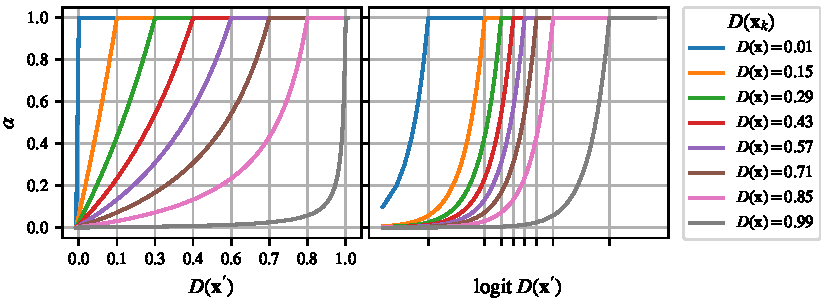
\includegraphics[width=\textwidth]{figures/alpha2.pdf}
    \caption{{\small
    We show the acceptance probabilities $\accept$ from~\eqref{eq:alpha from D} across different values for the discriminator score of the current state $D(\vec x_k)$ and the discriminator score of the proposed state $D(\vec x')$.
    On the right, we plot the curves in logit scale to allow closer examination of the limiting cases with $D$ close to zero and one.
    Small values of $D(\vec x_k)$ result in a linear ramp while large values of $D(\vec x_k)$ can be approximated as a step function.
    }}
    \label{fig:alpha}
\end{figure}

% Cherry picking approximation
\paragraph{Deterministic approximation}
It is also possible to replace the Markov chain with a deterministic approximation that is more parallelizable.
In Figure~\ref{fig:alpha} we show the acceptance probabilities for different discriminator scores of the current state $D(\vec x_k)$ and the proposal $D(\vec x')$.
The qualitative behavior of the curves are easily summarized.
In all curves, if $D(\vec x') \geq D(\vec x_k)$ then $\vec x'$ is always accepted.
As $D(\vec x_k) \rightarrow 0$ the region where $D(\vec x') < D(\vec x_k)$ becomes a linear ramp; and as $D(\vec x_k) \rightarrow 1$ it becomes a step function.
If $\PG$ and $\PR$ are well separated (which is believed to often be the case in GANs~\citep{Arjovsky2017}), and $D$ is near perfect, then $D(\vec x_0) \approx 1$: The acceptance probability becomes a step function if $\vec x_0 \sample \PR$.
Therefore, $D(\vec x_k)$ will stay near one and the acceptance function will be step function like.
In this scenario, we can approximate, $\accept(\vec x', \vec x_k) \approx \I\{D(\vec x') > D(\vec x_k)\}$, and therefore $G'$ takes the sample in the chain with the maximum score $D$.
However, this is with the provision that we beat the score of a randomly chosen sample of real data $D(\vec x_0)$.
This maximum procedure is a reduction and is therefore easily parallelizable.
The other advantage of this approximation is that it is invariant to monotonic transformation in the discriminator scores $D$ and therefore negates the need for calibration.

% Maybe Importance sampling also an option to include

\section{Results}

%We use an illustrative toy examples and real GANs on real data to illustrate the improvements made by the wrapped classifier $G'$.
%\subsection{Toy Data}
%We first demonstrate the MGAN on the toy two Gaussians example presented in~\citet{Arjovsky2017}.
%Figure~\ref{} shows how the convergence of samples to the true distribution over MCMC iterations.
%Note that if we don't strictly require all chains to end with a synthetic sample then the MGAN samples match the true distribution exactly at any number of MCMC iterations $K$.

\begin{figure}
    \centering
    \begin{subfigure}[b]{0.49\textwidth}
       \centering
       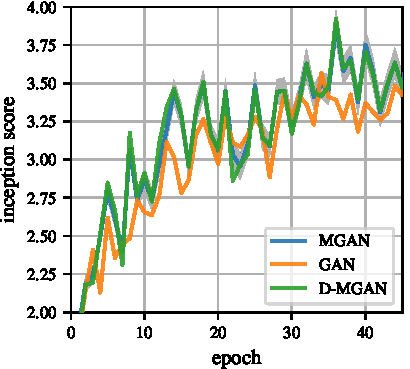
\includegraphics[width=2.75in]{figures/base_iso.pdf}
       \caption{performance by epoch}
       \label{fig:incep_by_epoch}
    \end{subfigure}
    \begin{subfigure}[b]{0.49\textwidth}
       \centering
       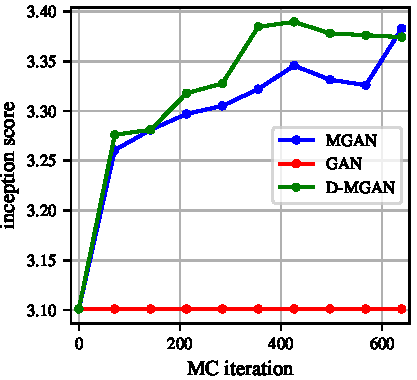
\includegraphics[width=2.75in]{figures/plot_per_mh.pdf}
       \caption{performance by MCMC iteration}
       \label{fig:incep_by_iter}
    \end{subfigure}
    \caption{{\small
        \todo{replot with standard colors for GAN vs. MGAN vs. D-MGAN (and/or remove D-MGAN).}
    Results of the MGAN experiments on CIFAR-10 using the DCGAN\@.
    On the left, we show the inception score by training epoch of the DCGAN\@.
    The error bars on MGAN performance (in grey) are computed using a t-test on the variation per batch across different splits of the inception score.
    On the left we show the inception score as a function of the number of MCMC iterations $K$ for the GAN at epoch 15.
    }}
\end{figure}

%\subsection{Real Data}

For real data experiments we considered three different data sets: CelebA~\citep{Liu2015}, CIFAR-10~\citep{Torralba2008}, and LSUN~\citep{Yu2015}.
We consider the traditional DC-GAN~\citep{Radford2015} and the popular WGAN~\citep{Arjovsky2017}\@.
We first examine the performance of the discriminator on held out data with and without calibration for DC-GAN\@.
For WGAN we can only use the calibrated discriminator as it does not output a probability.
% Look at losses for discriminator
%    maybe rescale all loses to 0-1 scale for plotting
We also show the results of the calibration statistic $Z$ from~\eqref{eq:calib score}.
These results confirm our expectation that the raw discriminators do not output well calibrated probabilities.

\begin{figure}
    \centering
    \begin{subfigure}[b]{0.49\textwidth}
       \centering
       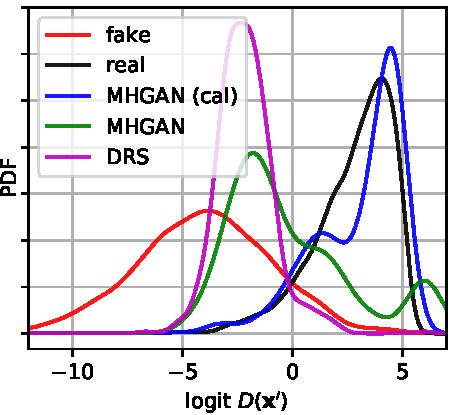
\includegraphics[scale=0.9]{figures/score_dist_overlap.pdf}
       \caption{epoch 13 scores}
       \label{fig:score_dist_overlap}
    \end{subfigure}
    \begin{subfigure}[b]{0.49\textwidth}
       \centering
       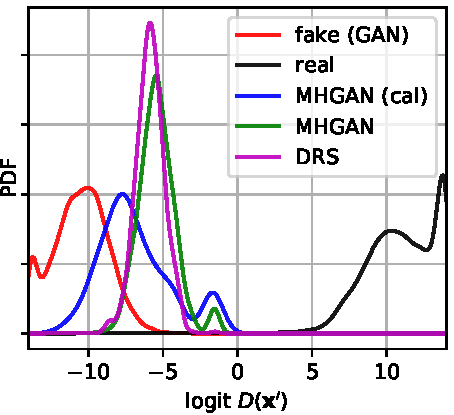
\includegraphics[scale=0.9]{figures/score_dist_no_overlap.pdf}
       \caption{epoch 14 scores}
       \label{fig:score_dist_no_overlap}
    \end{subfigure}
    \caption{{\small
    The distribution on discriminator scores at different training epochs for DCGAN on CIFAR-10 data set.
    On the right we show the scores at epoch 13 where there is some overlap between the scores of fake and real images.
    At epoch 14, on the left, the distributions are far apart even in logit scale.
    When there is overlap MGAN can correct the $\PG$ distribution to have scores looking similar to the real data.
    The deterministic approximation also fixes the distribution, but results in too much mass near the mode.
    However, when the distributions are too seperated the generator $G$ is essentially unfixable.
    In this case, the deterministic approximation can be used in place of the proper MGAN\@.
    }}
\end{figure}

% Look at incep score over 3 method on 3 data sets per epoch
% Can also show results by MH iteration
% DC GAN, WGAN, PGAN
% Use JY scatter plot
To evaluate the performance of the resulting wrapper generator $G'$, we plot inception scores per epoch in Figure~\ref{fig:incep_by_epoch}.
We see a consistent and statistically significant boost in inception score from $G'$ above $G$.
The actual gap of improvement made by MGAN oscillates from one epoch to the next.
This makes sense as we rely on $D$ being ``ahead'' in some sense.
Because GAN training is a game or sorts, how far ahead $D$ is will vary by epoch.

In Figure~\ref{fig:incep_by_iter} we also plot the inception score per epoch after $K=640$ MCMC iterations.
We see that most of gains are made in the first $k=100$ iterations, but smaller gains continue up to iteration $k=400$.

% TODO fill in XXX
We summarize the performance across all base GANs and data sets in Table~\ref{}.
The DCGAN is run to XXX epochs while the WGAN is run until XXX epochs.
In all cases we ran the MCMC procedure $K=640$ iterations as in Figure~\ref{fig:incep_by_iter}.
We see the same qualitative behavior as in Figure~\ref{fig:incep_by_epoch} with the MGAN correction providing a siginificant boost in inception score.

% Look at distn on D to make look more like real
%   both on synth and real
We also consider the distribution on discriminator scores.
In Figure~\ref{fig:score_dist_overlap}, the distributions on scores from real and fake images are well separated, but still contain \emph{some overlap}.
We can see that MCMC shifts the distribution of the fakes to match the distribution on true images.
In this case, our deterministic approximation focuses too much on the mode as a result of the overlap, but still makes an improvement over the base generator $G$.

\begin{figure}
    \centering
    \begin{subfigure}[b]{0.49\textwidth}
       \centering
       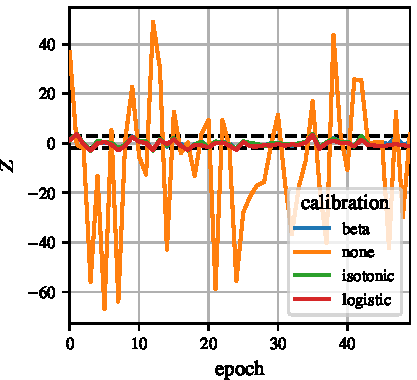
\includegraphics[scale=0.9]{figures/disc_calib.pdf}
       \caption{calibration $Z$}
       \label{fig:calibration stat}
    \end{subfigure}
    \begin{subfigure}[b]{0.49\textwidth}
       \centering
       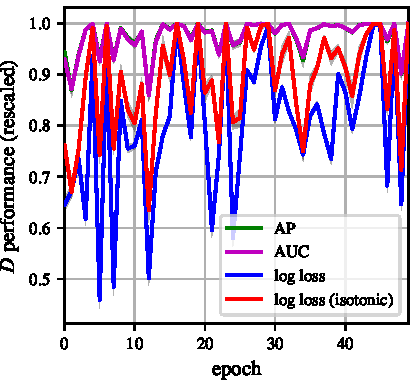
\includegraphics[scale=0.9]{figures/disc_perf.pdf}
       \caption{discriminator performance}
       \label{fig:discriminator_perf}
    \end{subfigure}
    \caption{{\small
    On the left we show the calibration statistic $Z$ for the discriminator for the DCGAN on CIFAR-10.
    The raw discriminator is clearly miscalibrated.
    All the calibration methods give roughly equivalent results.
    The left shows the predictive performance of the discriminator.
    The various performance metrics have been rescaled so a perfect classifier has score 1 and random classifier has score 0.5.
    The calibrated discriminator has higher predictive performance, but the oscillations are highly correlated with the ranking based performance metrics (AUC and AP)\@.
    Most of the variation from epoch to epoch is not merely differences in calibratedness.
    }}
    \label{fig:calibration}
\end{figure}

In Figure~\ref{fig:calibration} we show how calibration of the discriminator is necessary based on its raw performance.
Therefore, it is not surprising that it improves performance when used for the MGAN\@.

% Qualitative examples
% Finally, in Figure~\ref we show some qualitative examples of samples comparing the base generator $G$ and the improved MCMC version $G'$.

\section{Discussion}

% How many MH iters usually needed, what about computation burden
The wrapped GAN $G'$ will indeed have $K$ times the computational burden of $G$ when drawing samples; and Figure~\ref{fig:incep_by_epoch} shows improvements can be made even for smaller values of $K$.
However, the large computational burden of GANs is during training not when drawing samples (test)\@.
Therefore, in applications where the test speed is not the bottleneck, the wrapped GAN $G'$ is a good option.

% What does cherry picking perf say about distns in question
%    examples for resampling when overlap and no overlap
%    how it effects cherry pick approx
The deterministic approximation often has very similar behavior and performance to the full MGAN\@.
This validates the common view that base of support between $\PG$ and $\PR$ have little overlap.
% Implications on how it can be applied more generally
%   Will be most interesting cases where might be some overlap
However, applications where there is non-negligible overlap between $\PG$ and $\PR$ are perhaps the most interesting because proper calibration of the acceptance probabilities $\accept$ are the most critical in these cases.

% Generally interesting notes on calibration and side disc
%   And that D is always so good
Along these lines, we have shown the raw discriminators in GANs are poorly calibrated.
This is not a large surprise, but to our knowledge is the first time research has evaluated the discriminator in this way.

% Might need to consider stopping rule
A direction for possible future extensions to this work include finding appropriate stopping rules for the MCMC chain that introduce minimal bias.
In our setup, we must run the chain until at least receiving a single accept.
However, ending the chain at the first accept can potentially introduce a bias into the resulting distribution; This requires us to run the chain until a fixed, but perhaps too large, number of iterations $K$.

\section{Conclusions}

% usual wrap up BS paragraph
We have presented a way to incorporate the knowledge embedded in the discriminator $D$ into an improved generator $G'$ in a principled manner using MCMC methods.
Our method is based on the premise that the discriminator $D$ is essentially ``ahead'' of the generator $G$.
The principled MCMC setup stochastically selects among samples from $G$ to correct biases in the generator $G$.
This requires some modification to the MCMC equations as the neither the densities $\PG$ nor $\PR$ are available.
This method can perform the final coordinate descent move to optimize $G$ assuming $D$ is near perfect.
Further improvements for fancier proposals can potentially make these results possible with even shorter chains $K$.

\bibliographystyle{abbrvnat}
\bibliography{mgan_refs} % References file

\end{document}

